\chapter{Model Selection}
\label{ch:ch4cv}

\section{Model selection}
We tried different families of models by cross-validating them reusing the code that we did for HW2. Then, we tested the best model on these runs with on the quiz set, until we concluded that no classifier would beat the \verb|TreeBagger| classifier. There had been 2-cv rounds, using the following classifiers: 

\begin{itemize}
\item[\textit{1}]: \verb|averaged_perceptron|, \verb|LR|, \verb|LDA|, \verb|QDA|.
\item[\textit{2}]: \verb|AdaBoostM1|, \verb|LogitBoost|, \verb|GentleBoost|, \verb|RobustBoost|.
\end{itemize}

\section{Model hyperparameter selection}
Hyperparameters for the models were chosen using 2,5 and 10-fold cross validation on the dataset, using the quiz as testing set.
For our final model, which implements a \verb|TreeBagger| classifier, we used as hyperparameters: 
\begin{itemize}
    \item[\textit{iter}] which in this case stands for the number of trees used for the random forests.
    \item[\textit{npred}] which is the number of predictor or feature variables to select at random for each decision split, as described in the previous section.
\end{itemize}

Computation times for cross-validation were high, so we decided to output partial results on an incremental \textit{.csv} file. A plot displaying the relationship between the \textit{iter} and \textit{npred} parameters with respect to the cv error is shown below: 

\begin{center}
  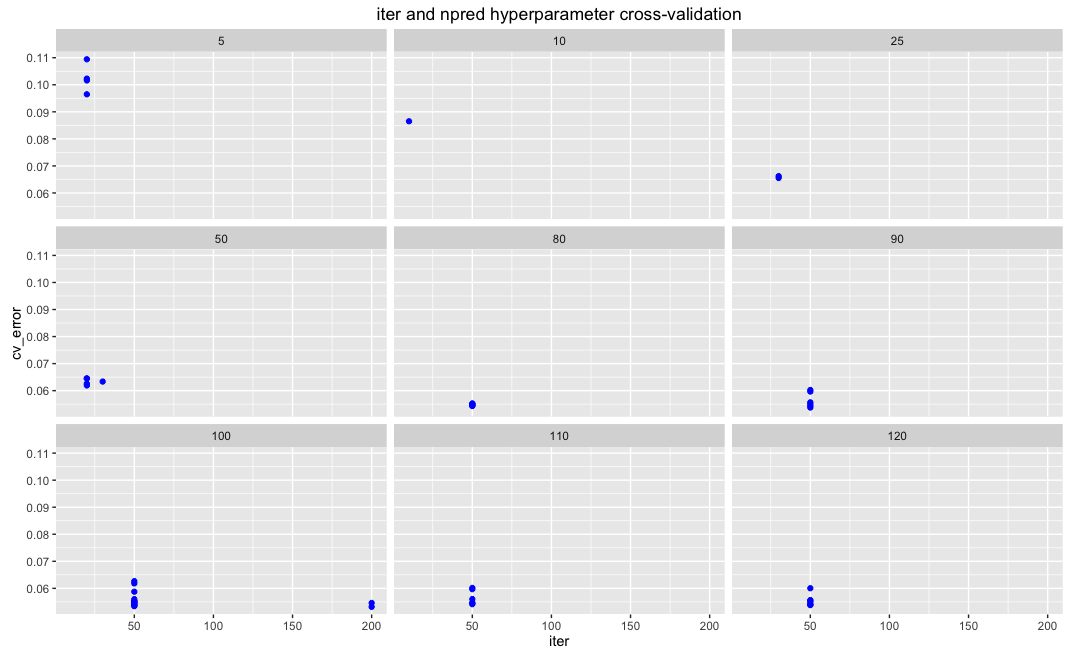
\includegraphics[scale=0.35]{./cv.png}
\end{center}    



